
\documentclass[12pt,epsfig,color,russian]{article}
\usepackage[russian]{babel}
\usepackage{epsfig}
\usepackage{color}

\topmargin=0cm
\hoffset -30mm
\voffset -12mm
\setlength{\unitlength}{1mm}
\parindent=10mm
\textheight=250mm
\textwidth=185mm
\pagestyle{empty}

\begin{document}
\sf\Large

\centerline{\LARGE\bf МОЛЕКУЛЯРНАЯ ФИЗИКА}
\vspace{5mm}
\centerline{\bf ГАЗЫ}
\vspace{5mm}
\noindent
``Атомный вес'' -- относительная масса атома (Джон Дальтон, 1803)\\
``Молекулярный вес'' -- относительная масса молекулы\\
Что считать за ЕДИНИЦУ массы?
\begin{center}
{\fbox{1 а.е.м. $\equiv$ M($^{12}$C)/12
= 1.6605402$_{10}\cdot10^{-24}$ г
= 931.494028$_{23}$ МэВ/c$^2$}}
\end{center}
(Раньше была ``кислородная'' а еще раньше -- ``водородная'' единица)\\
``Грамматом'' -- такое количество данного элемента, масса которого, вы\-ра\-жен\-ная в граммах, численно равна его атомному весу.\\
``Граммолекула'' $\equiv$ моль -- такое количество данного вещества, масса ко\-то\-ро\-го, выраженная в граммах, численно равна его молекулярному весу.\\
 $\Rightarrow$ Грамматом любого элемента содержит одно и то же число атомов, а граммолекула -- число молекул. Какое? Ответ: число Авогадро N.
\begin{center}
{\fbox{N = 6.02214179$_{30}\cdot10^{23}$ 1/моль}} -- сейчас-то знаем!
\end{center}
Итальянский граф Lorenzo Romano Amedeo Carlo Avogadro di Quaregna e Cerreto -- учитель физики в гимназии (1811): при одинаковых условиях в равных объемах газов содержится одинаковое число молекул. (Позднее стал профессором физики в Туринском университете).

Роберт Браун (R.Brown), 1827 г.: $\exists$ движение макрочастиц под ударами отдельных молекул $\Rightarrow$ молекулы $\exists$ и они не такие уж безумно малые.
% \vspace{-2mm}
  \begin{picture}(190,45)(0,0)
   %\put(0,0){\framebox(190,45)[b]{}}
   \put(125,0){\includegraphics{GP008F01.eps}}
   \put(0,0){\makebox(0,0)[bl]{\parbox{120mm}{
    Прикинем, каковы размеры 1 молекулы воды:\\
    молекулярный вес $\mu$(H$_2$O)$\simeq18$ г/моль\\
 $\Rightarrow$ масса $m=\mu/N\simeq3\cdot10^{-23}$ г\\
 $\Rightarrow$ объем $V=\rho m\simeq3\cdot10^{-23}$ см$^3$\\
 $\Rightarrow$ ``диаметр'' $d\sim\sqrt[3]{V}\simeq3.1\cdot10^{-8}$ см = 3.1 {\AA}
   }}}
  \end{picture}
\\
Во всяком веществе $\exists$ непрерывное хаотичное движение молекул, зависящее лишь от температуры. Точнее, температура -- это и есть мера хаотичного движения молекул. {\bf Молекулярно-кинетическая теория.}

Но сначала рассмотрим эмпирические закономерности в газах.


\underline{\bf Закон Бойля-Мариотта} (частный случай з.М-К)\\
Свойство газов: они целиком занимают сосуд, в котором заключены, и давят на стенки.
{\bf Давление} -- физ. величина = силе, действующей нор\-маль\-но на единицу площади:\vspace{-3mm}
\begin{displaymath}
p=\frac{f_n}{S}\vspace{-3mm}
\end{displaymath}
  \begin{picture}(185,45)(0,0)
   %\put(0,0){\framebox(185,45)[b]{}}
   \put(0,0){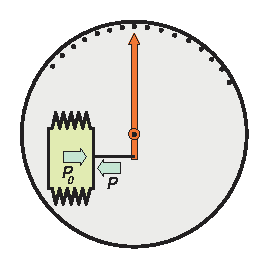
\includegraphics{GP008F02.eps}}
   \put(170,0){\includegraphics{GP008F03.eps}}
   \put(105,22){\makebox(0,0)[c]{\parbox{120mm}{
 Приборы для измерения давления под\-раз\-де\-ля\-ют\-ся по диапазону:
 барометры ($P\!\sim\! 1$ ат.), ма\-но\-мет\-ры ($P>1$ ат.),
 вакуумметры ($P<1$ ат.);
  по конструкции: анероиды, жидкостные (ртутные), пьезоэлектрические, ...
   }}}
  \end{picture}\\

Единицы измерения давления:
\begin{itemize}
\item CGS: $[f]$= дина, $\;\;[S]$= см$^2\;\;\;\;\Rightarrow\;\;\;[p]$= дина/см$^2$
\item SI:  $[f]$= Н, $\;\;[S]$= м$^2\;\;\;\;\Rightarrow\;\;\;[p]$= Паскаль = Н/м$^2$ = 10 дин/см$^2$
\item (несистемная): 1 мм ртутного столба (1 Торр)
\item (несистемная): 1 атмосфера = 760 мм рт.ст. $\simeq 1.013\cdot10^5$ Па
\item (несистемная): 1 бар = $10^5$ Па $\simeq$ 0.987 ат.
\item (допотопная): 1 PSI = 1 Pound per Square Inch (фунт на кв.дюйм)
\end{itemize}\vspace{5mm}

Итак, шотландец Robert Boyle (1662) и француз Edme Mariotte (1676)\\
  \begin{picture}(190,60)(0,0)
   %\put(0,0){\framebox(190,60)[b]{}}
   \put(0,0){\includegraphics{GP008F04.eps}}
   \put(65,57){\makebox(0,0)[tl]{\parbox{125mm}{
 независимо друг от друга обнаружили, что для данной массы газа при постоянной температуре давление газа меняется обратно пропорционально его объему (т.е., газы -- упруги!):
\begin{center}
\fbox{$pV=$const}
\end{center}
При очень больших давлениях это перестает работать (до нуля газ не сжимается).
   }}}
  \end{picture}
\newpage

Другой важный параметр -- {\bf температура}. Многие свойства тел ме\-ня\-ют\-ся при нагревании $\Rightarrow$ можно их использоать для измерения $T$. Рас\-ши\-ре\-ние жидкости: ртутный и спиртовой термометры; расширение твер\-до\-го тела: биметаллический термометр; электрические свойства: термо\-пара, термистор; излучательные свойства: пирометр.

Единица измерения -- 1 градус. Какой? Градусы бывают разные...
\begin{itemize}
\item Шкала Реомюра: Франция, 1730. Уже давно не используется.
 \begin{displaymath}
 \left\{
 \begin{array}{cl}
 1^\circ\equiv & \left[T(\texttt{кипения воды})-T(\texttt{таяния льда})\right]/80\\
 0R\equiv &T(\texttt{таяния льда})
 \end{array}
 \right.
 \end{displaymath}
\item Шкала Цельсия: Швеция, 1742. Широко используется в быту.
 \begin{displaymath}
 \left\{
 \begin{array}{cl}
 1^\circ\equiv & \left[T(\texttt{кипения воды})-T(\texttt{таяния льда})\right]/100\\
 0C\equiv &T(\texttt{таяния льда})
 \end{array}
 \right.
 \end{displaymath}
\item Шкала Фаренгейта: Германия, 1724. Используется только в США, Канаде и Ямайке.
 \begin{displaymath}
 \begin{array}{rl}
 1) &
 \left\{
 \begin{array}{cl}
 1^\circ\equiv & \left[T(\texttt{тела человека})-T(\texttt{таяния льда с солью})\right]/100\\
 0F\equiv &T(\texttt{таяния льда с солью})
 \end{array}
 \right.
 \\ \\
 2) &
% \end{displaymath}
% \begin{displaymath}
 \left\{
 \begin{array}{cl}
 1^\circ\equiv & \left[T(\texttt{кипения воды})-T(\texttt{таяния льда})\right]/180\\
 32F\equiv &T(\texttt{таяния льда})
 \end{array}
 \right.
 \end{array}
 \end{displaymath}
\item Абсолютная шкала. Единица -- 1 Кельвин (названа в честь англ. физика Дж.Томсона (=лорд Кельвин). Используется в науке.
 \begin{displaymath}
 1K\equiv \left[T(\texttt{кипения воды})-T(\texttt{таяния льда})\right]/100
 \end{displaymath}
\end{itemize}
\begin{center}
\begin{tabular}{|l||c|c|c|}\hline
Явление с характерной  & Абс.шкала &  Цельсий     & Фаренгейт  \\
 температурой          &   $K$     & $^\circ C$   & $^\circ F$ \\ \hline\hline
Абсолютный ноль        & $  0   $    & $-273.15 $   & $-459.67$    \\ \hline
Кипение азота          & $ 77.4 $    & $-195.75 $   & $-320.35$    \\ \hline
Плавление льда с солью & $255.37$    & $ -17.78 $   & $   0   $    \\ \hline
Плавление льда         & $273.15$    & $   0    $   & $ +32   $    \\ \hline
Тело человека          & $\sim310$   & $\sim+36.6$   & $ +98.2 $    \\ \hline
Кипение воды           & $373.15$    & $+100    $   & $  212  $    \\ \hline
\end{tabular}
\end{center}

1877 г. Международный Комитет мер и весов: {\bf Постулировалось}, что давление \underline{\bf линейно} меняется с температурой:
\fbox{$p_t=p_0(1+\alpha t)$} -- и было предложено это и использовать как термометр. Для шкалы Цельсия коэф-т $\alpha$ оказался $\simeq0.0036613$ град$^{-1}$. Сегодня известно, что выбор был удачным: H$_2$ действительно ведет себя по этой формуле в широком $T$-диапазоне.  Как ведут себя остальные газы?

Эмпирические \underline{\bf законы Гей-Люссака} (Joseph Louis Gay-Lussac, 1778-1850):
\begin{enumerate}
\item при постоянном объеме и массе газа его давление $\propto$ температуре

      \fbox{$p_t=p_0(1+\alpha_p t)$}, где $\alpha_p$ -- термический коэффициент давления
\item при постоянном давлении и массе газа его объем $\propto$ температуре

      \fbox{$V_t=V_0(1+\alpha_vt)$}, где  $\alpha_v$ -- термический коэф-т объемного расширения
\end{enumerate}
Второй закон еще называют законом Шарля (Jaques Charles, 1746-1823; изобрел водородный воздушный шар).


Для водорода эти 2 закона выполняется точно (по определению), а для остальных -- не очень. Например, $pV=$const., $\alpha_p=\alpha_v$\\

\begin{tabular}{|c||c|c|c|c|c||c||c|}\hline
        & \multicolumn{5}{|c||}{$pV$}& $\alpha_p$& $\alpha_v$\\ \cline{2-6}
Газ     & 1 ат & 100 ат & 200 ат & 500 ат & 1000 ат & $\times10^3$ & $\times10^3$\\ \hline \hline
H$_2$   & 1.0000 & 1.0690 & 1.1380 & 1.3565 & 1.7200 & 3.6613 & 3.6600 \\ \hline
N$_2$   & 1.0000 & 0.9941 & 1.0483 & 1.3900 & 2.0685 & 3.6744 & 3.6732 \\ \hline
O$_2$   & 1.0000 & 0.9265 & 0.9140 & 1.1560 & 1.7355 &        &        \\ \hline
воздух  & 1.0000 & 0.9730 & 1.0100 & 1.3400 & 1.9920 & 3.6750 & 3.6760 \\ \hline
CO$_2$  &        &        &        &        &        & 3.7262 & 3.7414 \\ \hline
He      &        &        &        &        &        & 3.6601 & 3.6582 \\ \hline
\end{tabular}\\

При очень больших давлениях отступления еще сильнее. Объем азота при 15 000 ат. в 16 раз больше расчетного.\\
  \begin{picture}(190,100)(0,0)
   %\put(0,0){\framebox(190,100)[b]{}}
   \put(0,60){\includegraphics{GP008F05.eps}}
   \put(0,0){\includegraphics{GP008F06.eps}}
   \put(100,100){\makebox(0,0)[tl]{\parbox{85mm}{
  По закону Гей-Люссака, все изо\-хо\-ры для разного количества газа пересекаются в одной точке. Для разных газов -- тоже. Эта особая точка соответствует $t=-273^\circ$C. Изобары ведут себя так же.

  \hspace{8mm}Если абстрагироваться от воз\-мож\-ных небольших от\-кло\-не\-ний, то в первом приближении законы Б-М и Г-Л соблюдаются хорошо.

  \hspace{8mm}\underline{\bf Идеальный газ} --
  гипо\-те\-ти\-чес\-кий газ, для которого они выполнялись бы \underline{строго}.
   }}}
  \end{picture}\\
Если перейти к абсолютной температуре $t\rightarrow T$ (то есть, от градусов Цельсия к Кельвинам), то все уравнения упрощаются

Бенуа Поль Эмиль Клапейрон (1834):
\begin{equation}
\frac{pV}T=\texttt{const.}
\end{equation}
здесь константа зависит от того, сколько взято газа и какого. Как уже говорилось, по закону Авогадро, моль любого газа при одинаковых усло\-ви\-ях занимает один и тот же объем. {\bf Молярный объем}: $V_0$ -- объем, занима\-е\-мый одним молем газа.\\
Д.И.Менделеев (1874) все это объединил и получил уравнение Клапейрона-Менделеева, то есть,  \fbox{\bf уравнение состояния идеального газа}:\\
\begin{equation}
pV_0=RT
\end{equation}
$R$ -- Универсальная газовая постоянная. Чему она равна? Посчитаем:\\
 $R=pV_0/T\simeq 1$ ат $\cdot 22.4$ л / 273 град. $\simeq$ 0.082 л ат/град/моль\\

Более точно:
\fbox{$R=8.31441_{26}$ Дж/моль/К =$8.31441_{26}\cdot10^7$ эрг/моль/К}\\

Если у нас не 1 моль газа, а, например, $m$ граммов при молекулярном весе $\mu$, то формула несколько изменится. $m$ граммов -- это $\frac m\mu$ молей, и они занимают объем $V=V_0\cdot\frac m\mu$, поэтому
\begin{displaymath}
pV=\frac m\mu RT
\end{displaymath}
Например, найдем плотность воздуха при 1 атмосфере и 27$^\circ$C:
\begin{displaymath}
\rho=\frac mV =\frac {p\mu}{RT} = 1\texttt{ат}\cdot\frac{29\texttt{ г}}{\texttt{моль}}\cdot
       \frac{\texttt{град моль}}{0.082\texttt{л ат}}\cdot\frac1{300 \texttt{град}}
       \simeq1.17\frac{\texttt{г}}{\texttt{л}}=1.17\frac{\texttt{кг}}{\texttt{м}^3}
       =1.17\frac{\texttt{мг}}{\texttt{см}^3}
\end{displaymath}
То есть, плотность газов $\sim$ на 3 порядка < плотности воды.

Еще задачка: сколько нужно молей водорода, чтобы наполненный им шар смог поднять человека? $\mu(H_2)$=2, а для воздуха $\mu$=29, поэтому выталкивающая сила = $\frac{29-2}{29}$ от веса воздуха. Считая, что масса человека + масса оболочки = 100 кг, и вспомнив, что 1 м$^3$ воздуха весит 1.17 кг, получим, что водородный шар объемом 1 м$^3$ может поднять $\frac{29-2}{29}\cdot1.17\simeq1.09$ кг, а для поднятия 100 кг нужно, соответственно, 92 м$^3$ ($\oslash$ 5.6 м) или $\frac{92000}{22.4}\cdot\frac{273}{300}\simeq3738$ молей. Если пытаться получить водород из реакции
\begin{displaymath}
2HCl+Zn\rightarrow ZnCl_2+H_2
\end{displaymath}
то нужно 250 кг цинка и 270 кг соляной кислоты. Лучше сразу забыть и купить на сэкономленные деньги авиабилет.\\ \\

\underline{\bf Основные представления кинетической теории газов.}

Поскольку при н.у. газы в 1000 раз менее плотны, чем жидкости, то расстояния между молекулами в $\sqrt[3]{1000}\simeq10$ раз больше их размеров. Молекулы упруго соударяются друг с другом и со стенками. $\Rightarrow$ распро\-стра\-не\-ние на весь объем и диффузия. Удары по стенкам $\Rightarrow$ давление (идея Д.Бернулли, 1738, СПб). Дальнейшее развитие -- лишь во второй половине XIX века. (Клаузиус, Больцман, Максвелл).\\
  \begin{picture}(190,51)(0,0)
   %\put(0,0){\framebox(190,51)[b]{}}
   \put(0,0){\includegraphics{GP008F07.eps}}
   \put(55,52){\makebox(0,0)[tl]{\parbox{135mm}{
   Рассмотрим маленький кубический объем $V$=$L^3$ с $n$ молекулами. Считаем, что $\frac n3$ молекул летает $\parallel$ оси $x$ между левой и правой стенками, $\frac n3$ -- $\parallel$ оси $y$ между передней и задней, и  $\frac n3$ -- $\parallel$ оси $z$ между верхней и нижней стенками. При упругом ударе об стенку молекула передает ей импульс $2mv$. Период ударов -- это время, чтобы слетать туда и обратно: $\Delta t=2L/v$.
    }}}
  \end{picture}\\
Регулярная мгновенная передача импульса $2mv$ с периодом $\Delta t$ равносильна тому, как если бы в течение этого времени действовала постоянная малень\-кая сила $\Delta f$, сообщающая стенке тот же импульс за то же время: $\Delta f\cdot \Delta t = 2mv$. Подставив значение $\Delta t=2L/v$, получим для вклада от одной i-ой молекулы: $\Delta f_i=mv_i^2/L$. Если у нас имеется $j=n/3$ таких молекул, каждая с какой-то своей скоростью, то суммарное давление на стенку определится суммой всех сил $\Delta f_i$:
\begin{displaymath}
p=\frac FS=\frac{\sum_{i=1}^{j}\Delta f_i}{L^2}=\frac 1{L^3}\sum_{i=1}^{j}mv_i^2
\end{displaymath}
Обратим внимание, что среднюю кинетическую энергию молекул можно определить как\vspace{-4mm}
\begin{displaymath}
\overline{w}=\frac 1{j}\sum_{i=1}^{j}\frac{mv_i^2}2
\end{displaymath}
Тогда предыдущее выражение превращается в $p=\frac{2j}{L^3}\overline{w}$, а если обозначить за $n_0$ число молекул в единице объема: $n_0=n/L^3=3j/L^3$,  то
\begin{displaymath}
p=\frac23\;n_0\;\overline{w}\hspace{10mm}\texttt{-- основная формула кинетической теории газов}
\end{displaymath}
Если домножим обе части на молярный объем и учтем, что $n_0V_0=N$, то
\begin{displaymath}
pV_0=\frac23\;N\;\overline{w}\hspace{20mm}\texttt{но из ур.К-М:}\hspace{10mm}pV_0=RT
\end{displaymath}
поэтому можно выразить значение средней энергии через температуру:
\begin{equation}
{\color{green}\overline{w}}=\frac32\;\frac RN\;T={\color{green}\frac32\;k\;T}
\end{equation}
где $k=R/N$ -- постоянная Больцмана (Ludwig Eduard Boltzmann, 1844-1906, Вена)\\
\begin{displaymath}
\texttt{Численное значение: }k=\left\{
\begin{array}{ll}
1.3806504_{24}\cdot 10^{-23} & \texttt{Дж/К}\\
1.3806504_{24}\cdot 10^{-16} & \texttt{эрг/К}\\
8.617343_{15}\cdot 10^{-5}&\texttt{эВ/К}
\end{array}\right.
\end{displaymath}
Посмотрим, сколько молекул в единице объема при н.у.:
\begin{displaymath}
n_0=\frac{p}{kT}=2.6867774_{47}\cdot10^{25}\texttt{м}^{-3}
=2.6867774_{47}\cdot10^{19}\texttt{см}^{-3}\texttt{ -- число Лошмидта}
\end{displaymath}
\\

Итак, важный вывод:\\
\underline{\bf температура однозначно определяется средней кинетической}\\
\underline{\bf энергией поступательного движения молекул.}\\ \\
Задача: какова средняя энергия и скорость молекул N$_2$ при разных $T$ ?\\
Решение:
\begin{displaymath}
\overline{w}=\frac32\;k\;T,\;\;\;\;v_T\equiv\sqrt{\overline{v^2}}
=\sqrt{\frac{2\overline{w}}{m}}
=\sqrt{\frac{3kT}{m}}
=\sqrt{\frac{3RT}{mN}}
=\sqrt{\frac{3RT}{\mu}}
=\sqrt{\frac{3kNT}{\mu}}
\end{displaymath}
\begin{displaymath}
\begin{array}{crrlrr}
T=&0.01K: &\hspace{10mm} \overline{w}=&1.29\texttt{ мкэВ}&\hspace{10mm}v_T=&3\texttt{ м/с}\\
T=&4K:    & \overline{w}=&0.52\texttt{ мэВ}&v_T=&60\texttt{ м/с}\\
T=&300K:  & \overline{w}=&0.04\texttt{ эВ}&v_T=&517\texttt{ м/с}\\
T=&5760K: & \overline{w}=&0.74\texttt{ эВ}&v_T=&2300\texttt{ м/с}
\end{array}
\end{displaymath}
\rule{185mm}{0.3mm}

\begin{displaymath}
\texttt{Вспомним основную формулу: }\hspace{10mm} p=\frac23\;n_0\;\overline{w}
\end{displaymath}
Что если молекулы -- не одинаковы? $n_0=n_{0A}+n_{0B}+n_{0C}+\ldots$ Каждый газ давит на стенки сам по себе, независимо от остальных. Поэтому

Закон Дальтона (John Dalton, 1766-1844, UK): Сумма {\bf парциальных} давлений идеальных газов равна давлению всей газовой смеси.
\begin{displaymath}
p=p_{A}+p_{B}+p_{C}+\ldots
\end{displaymath}
Следствие: если разные идеальные газы при одинаковых условиях (p,T) смешать, то давление не изменится, а объемы сложатся.\\

Мы видели, что $T$ -- это кинетическая энергия поступательного движе\-ния молекул. Но у молекул может быть еще {\bf энергия вращения}, а также {\bf энергия колебаний}!

\underline{\bf Число степеней свободы} -- число координат, необходимых для пол\-но\-го описания положения тела в пространстве. Для материальной ТОЧКИ хватит трех -- x,y,z. Для ТЕЛА надо еще 3: две для задания оси вращения ($\angle\vartheta$ и $\angle\varphi$), и одна -- для угла поворота $\angle\xi$. Если еще возможны смещения (колебания) отдельных частей тела, то для этого нужны еще дополнитель\-ные координаты.

Ни одно из движений не имеет преимущества $\Rightarrow$ ПРЕДПОЛОЖЕНИЕ:
{\bf На каждую степень свободы молекулы в среднем приходится одно и то же количество энергии $\bf \overline{w}/3=\frac12kT-\frac12\frac RNT$.}

Пусть газ имеет $i$ степеней свободы. Внутренняя энергия 1 моля газа:
$U_0=N\frac i2\frac RNT = \frac i2RT $ -- зависит только от $T$, но не от $V$ или $p$.\\

{\bf Удельная теплоемкость ($c$) и молярная теплоемкость ($C$)} -- количество тепла, которое надо сообщить 1 (кило)грамму или 1 молю вещества, чтобы его $T$ увеличилась на 1$^\circ$.
\begin{displaymath}
C=\mu c
\end{displaymath}
Результат, оказывается, зависит от того, {\bf КАК} происходит нагревание!\\

Например, нагреваем 1 моль газа при постоянном объеме $V$. Поскольку работа при этом не совершается, то все тепло идет на увеличение $U$:
\begin{displaymath}
\Delta U_0 =\frac i2R(T+1)-\frac i2RT = \frac i2R \hspace{20mm}\Rightarrow \hspace{10mm}
C_V=\frac i2R;\;\;c_V=\frac i2\frac R\mu
\end{displaymath}
Поскольку количество тепла принято измерять в калориях (1 г воды от 19.5 до 20.5 $^\circ$C), то $\exists$ соотношение: 1 кал $\approx$ 4.184 Дж. Можно пересчитать:
\begin{displaymath}
R=8.31441\texttt{ Дж/моль/К }\simeq1.986\texttt{ кал/моль/К}
\end{displaymath}
\newpage
\noindent
  \begin{picture}(190,60)(0,0)
   %\put(0,0){\framebox(190,60)[b]{}}
   \put(0,0){\includegraphics{GP008F08.eps}}
   \put(35,60){\makebox(0,0)[tl]{\parbox{155mm}{
Теперь нагреем 1 моль газа при постоянном давлении $p$. Газ расширится и сдвинет поршень на рассояние $h$, совершив работу $A=f\cdot h=p\cdot S\cdot h=p\cdot \Delta V$. Поскольку молярный объем при температуре $T$ составлял $V_0=RT/p$, а после нагрева до температуры $T+1$ стал $V_0'=R(T+1)/p$, то $\Delta V=R/p$, а совершенная работа $A=p\Delta V=R$.\\
Итак, при постоянном давлении теплоемкость выше, т.к. тепло идет не только на нагрев, но еще и на работу по расширению:
   }}}
  \end{picture}
\begin{displaymath}
C_p=C_V+R=\frac i2R+R=\frac{i+2}2R
\end{displaymath}
Если обозначить буквой $\gamma$ отношение теплоемкостей $C_p/C_V\equiv \gamma$, то видно, что оно зависит только от числа степеней свободы: $\gamma=\frac{i+2}i=1+2/i$. \\
Для одно-атомных молекул должно быть:\\
\hspace*{10mm}  $i=3\;\;\;C_V=\frac32R=2.98$ кал/моль/К; $C_p=\frac52R=4.97$ кал/моль/К\\
для двух-атомных:\\
\hspace*{10mm}  $i=5\;\;\;C_V=\frac52R=4.97$ кал/моль/К; $C_p=\frac72R=6.95$ кал/моль/К\\
для трех-атомных:\\
\hspace*{10mm}  $i=6\;\;\;C_V=\frac62R=5.96$ кал/моль/К; $C_p=\frac82R=7.94$ кал/моль/К\\
\begin{picture}(190,95)(0,0)
 %\put(0,0){\framebox(190,95)[b]{}}
 \put(20,10){\includegraphics{GP008F09.eps}}
 \put(90,0){\makebox(0,0)[bl]{\parbox{110mm}{
\begin{tabular}{|c||c|c||c|c|}\hline
газ          & $C_V$ & $C_p$ & $\gamma$ &  i   \\ \hline \hline
He           &  2.98 &  5.00 & 1.67     & 2.99 \\ \hline
Ar           &  2.98 &  5.07 & 1.65     & 3.07 \\ \hline \hline
H$_2$        &  4.87 &  6.87 & 1.41     & 4.88 \\ \hline
N$_2$        &  4.96 &  6.84 & 1.41     & 4.88 \\ \hline
O$_2$        &  4.99 &  6.90 & 1.38     & 5.22 \\ \hline
CO           &  5.01 &  7.01 & 1.40     & 5.01 \\ \hline \hline
H$_2$O       &  6.65 &  8.65 & 1.30     & 6.65 \\ \hline
CH$_4$       &  6.51 &  8.51 & 1.31     & 6.51 \\ \hline \hline
CHCl$_3$     & 15.2  & 17.2  & 1.13     & 15.2 \\ \hline
C$_2$H$_5$OH & 18.9  & 20.9  & 1.11     & 18.9 \\ \hline \hline
\end{tabular}
 }}}
\end{picture}\\
\begin{picture}(190,45)(0,0)
 %\put(0,0){\framebox(190,45)[b]{}}
 \put(0,0){\includegraphics{GP008F10.eps}}
 \put(90,0){\makebox(0,0)[bl]{\parbox{100mm}{
В действительности, теплоемкость рас\-тет с температурой. А с охла\-ж\-де\-ни\-ем степени свободы как бы "вымо\-ра\-жи\-ва\-ют\-ся". Причина: вращательная и колебательная энергии квантуются, и при низкой $T$ их просто нет. Колебания
 }}}
\end{picture}\\
 сказываются либо при совсем высокой $T$, либо при сложном строении молекул (тогда квант мал по величине). \\
\begin{picture}(190,55)(0,0)
 %\put(0,0){\framebox(190,55)[b]{}}
 \put(110,0){\includegraphics{GP008F11.eps}}
 \put(0,0){\makebox(0,0)[bl]{\parbox{100mm}{
 Например: двухатомный газ при комнатной $T$ имеет 5/2. При охла\-ж\-де\-нии сначала пропадает вращение (5/2$\rightarrow$3/2), а затем заз замерзает, и вообще движение пропадает (3/2$\rightarrow$0). При нагревании, наоборот, появляется возможность колебаний (5/2$\rightarrow$7/2).
 }}}
\end{picture}\\
Да еще происходит частичная диссоциация $\Rightarrow$ вместо одной 2-атомной молекулы с 7/2 возникают две 1-атомные (3/2+3/2=6/2)...\\

\end{document}
